%%%%%%%%%%%%%%%%%%%%%%%%%%%%%%%%%%%%%%%%%
% Short Sectioned Assignment
% LaTeX Template
% Version 1.0 (5/5/12)
%
% This template has been downloaded from:
% http://www.LaTeXTemplates.com
%
% Original author:
% Frits Wenneker (http://www.howtotex.com)
%
% License:
% CC BY-NC-SA 3.0 (http://creativecommons.org/licenses/by-nc-sa/3.0/)
%
%%%%%%%%%%%%%%%%%%%%%%%%%%%%%%%%%%%%%%%%%

%----------------------------------------------------------------------------------------
%	PACKAGES AND OTHER DOCUMENT CONFIGURATIONS
%----------------------------------------------------------------------------------------

\documentclass[paper=a4, fontsize=11pt]{scrartcl} % A4 paper and 11pt font size

\usepackage[T1]{fontenc} % Use 8-bit encoding that has 256 glyphs
\usepackage{fourier} % Use the Adobe Utopia font for the document - comment this line to return to the LaTeX default
\usepackage[english]{babel} % English language/hyphenation
\usepackage{amsmath,amsfonts,amsthm} % Math packages

\usepackage{lipsum} % Used for inserting dummy 'Lorem ipsum' text into the template
\usepackage{bbding}
\usepackage{multirow}
\usepackage{caption}
\usepackage{graphicx}
\usepackage{hyperref}
\usepackage{enumitem}

\usepackage{sectsty} % Allows customizing section commands
\allsectionsfont{\centering \normalfont\scshape} % Make all sections centered, the default font and small caps

\usepackage{fancyhdr} % Custom headers and footers
\pagestyle{fancyplain} % Makes all pages in the document conform to the custom headers and footers
\fancyhead{} % No page header - if you want one, create it in the same way as the footers below
\fancyfoot[L]{} % Empty left footer
\fancyfoot[C]{} % Empty center footer
\fancyfoot[R]{\thepage} % Page numbering for right footer
\renewcommand{\headrulewidth}{0pt} % Remove header underlines
\renewcommand{\footrulewidth}{0pt} % Remove footer underlines
\setlength{\headheight}{13.6pt} % Customize the height of the header

\numberwithin{equation}{section} % Number equations within sections (i.e. 1.1, 1.2, 2.1, 2.2 instead of 1, 2, 3, 4)
\numberwithin{figure}{section} % Number figures within sections (i.e. 1.1, 1.2, 2.1, 2.2 instead of 1, 2, 3, 4)
\numberwithin{table}{section} % Number tables within sections (i.e. 1.1, 1.2, 2.1, 2.2 instead of 1, 2, 3, 4)

\setlength\parindent{0pt} % Removes all indentation from paragraphs - comment this line for an assignment with lots of text

\usepackage{amsmath}

%----------------------------------------------------------------------------------------
%	TITLE SECTION
%----------------------------------------------------------------------------------------

\newcommand{\horrule}[1]{\rule{\linewidth}{#1}} % Create horizontal rule command with 1 argument of height

\title{	
\normalfont \normalsize 
\textsc{} \\ [25pt] % Your university, school and/or department name(s)
\horrule{0.5pt} \\[0.4cm] % Thin top horizontal rule
\huge Evaluation of Early Stopping in A/B Testing  \\ % The assignment title
\horrule{2pt} \\[0.5cm] % Thick bottom horizontal rule
}

\author{Shan Huang} % Your name

\date{\normalsize\today} % Today's date or a custom date

\begin{document}

\maketitle % Print the title

%----------------------------------------------------------------------------------------
%	PROBLEM 1
%----------------------------------------------------------------------------------------

This documentation presents the evaluation of early stopping algorithms. 

\section{Problem}
Given samples $\textbf{x}$ from treatment group, samples $\textbf{y}$ from control group, we want to know whether there is a significant difference between the means $\delta = \mu(y)-\mu(x)$.

To save the cost of long-running experiments, we want to stop the test early if we are already certain that there is a statistically significant result.

\section{Significance Decision}
\label{sec:byt}
We can decide whether the difference is statistically significant using either:

\begin{itemize}[noitemsep]
\item \textbf{Confidence interval}: If 0 is outside confidence interval of $\delta$, it is statistically significant.
\item or \textbf{credible interval}: Credible interval is the Bayesian version of confidence interval. If 0 is outside credible interval of $\delta$, it is statistically significant.
\item or \textbf{Bayes factor}: Theoretically, Bayes factors higher than 3 can be interpreted as support for the null hypothesis (significant no difference), whereas values smaller than 1/3 can be interpreted as support for the alternative hypothesis (significant difference). Values between 1/3 and 3 are inconclusive. \textbf{In our test, we will only use Bayes factor less than 1/3 as decision criteria}. See reasons below.
\end{itemize}

Given the null hypothesis $H_0$ representing no difference, the alternative hypothesis $H_1$ representing a difference of the means, the ability of each metric, i.e., types of significance it can detect, is shown in the following table.
\begin{center}
  \begin{tabular}{ | r | c | c | c | c | }
    \hline
    & Paradigm & Significant $H_1$ & Significant $H_0$ & No Significant Result \\ \hline
    \textbf{Confidence Interval} & frequentist &  \Checkmark &  & \Checkmark\\ \hline
    \textbf{Credible Interval} & Bayesian & \Checkmark &  & \Checkmark\\ \hline
    \textbf{Bayes factor} & Bayesian & \Checkmark & \Checkmark & \Checkmark\\
    \hline
  \end{tabular}
\captionof{table}{Comparison of decision ability}
\end{center}

To be consistent with all mehods, we draw a binary conclusion that either there is a significant difference or not. In other words, the first column means that there is a significant difference, combining the second and third column means that there is no significant difference. Thus, we only use the part where Bayes factor less than 1/3 as decision criteria.

It is worth noting that a \textbf{typical conclusion of Bayes factor} would be for instance "\emph{There is a significant difference corresponds to Cauchy prior and a threshold of Bayes factor=3}". This might be quite difficult to explain to non-tech users. On the other hand, a \textbf{conclusion based on interval} can be more intuitive such as "\emph{You can be 95\% sure that the significant difference is not due to chance}".


\section{Early Stopping Criteria}
We can stop the experiment by either
\begin{itemize}[noitemsep]
\item \textbf{Confidence interval}: Calculate the new significance level for each day based on alpha-spending function in group sequential method. Use new significance level to compute confidence interval. Stop the test if 0 is outside confidence interval of $\delta$. 
\item or \textbf{credible interval}: Stop the test if 0 is outside credible interval of $\delta$.
\item or \textbf{Bayes factor}: Stop the test if Bayes factor is smaller than 1/3.
\item or \textbf{Bayes precision}: Stop the test if credible interval width is smaller than 0.08. 
\end{itemize}


\section{Metric}

\subsection{Evaluate Significance Decision}
We are going to compare false positive (type I error), false negative (type II error), true positive, true negative rates for the three significance decision criteria described in Section ~\ref{sec:byt}. These metrics will be evaluated only on simulation data, where we know the true value of significance.

\subsection{Evaluate Early Stopping Criteria}
\label{sec:esc}
It is obvious that if we use frequentist's approach --- in our case is confidence interval --- for early stopping, we should also use frequentist's approach for significance decision. On the other hand, when using Bayes factor for early stopping, we find a conflicting result if we draw significance conclusion based on credible interval. Therefore we don't evaluate all combinations of early stopping algorithms and significance decisions, find below a table of combination we evaluated on.

\begin{center}
  \begin{tabular}{ | r | c | c | c | c | }
    \hline
    \multirow{2}{*}{Significant Based On} & \multicolumn{4}{ |c| }{Early Stopping Based On} \\ \cline{2-5}
    & Confidence Interval & Credible Interval & Bayes factor & Bayes precision \\ \hline
    Confidence Interval & \Checkmark & &  &  \\ \hline
    Credible Interval &  & \Checkmark &  &  \\ \hline
    Bayes factor &  & & \Checkmark & \Checkmark \\ \hline
  \end{tabular}
\captionof{table}{Combinations of early stopping and significance decision for evaluation}
\end{center}

For each combination shown in the table above, we compute the following metrics:
\begin{itemize}[noitemsep]
\item \textbf{False positive rate}: Percentage of tests which are wrongly stopped. i.e., Early stop says there is a significant difference and stops the test, but the test to the end day (as if there is no early stopping) will tell you it is not significant.
\item \textbf{Run time reduced (all)}: Percentage of run time reduced for all tests.
\item \textbf{Run time reduced (true positive)}: Percentage of run time reduced for only the correctly stopped tests.
\item \textbf{Bias}: Average difference of effect size (delta) between stopping day and end day of test (as if there is no early stopping).
\end{itemize}

\section{Evaluation}

The evaluation is conducted on both simulation data and real data. Code can be found \href{https://github.com/shansfolder/ABTestingEarlyStoppingEvaluation}{\underline{here}}.

\subsection{Simulation Data}
We generate 2000 simulation tests based on Gaussian distributed KPIs, of which 1000 tests have a significant difference between control and treatment, while the other 1000 tests have no significant difference. The effect size of significant difference satisfies the minimal detectable effect size from power analysis. 

We simulate the experiment data for a period of 20 days. We run an analysis and decide whether to stop on each day. The frequency of visits per entity is modelled by a Poisson distribution. It is simulated in a way that an entity will visit the experiment 3 times in average. 

First, the table below shows the performance of \textbf{significance decision} algorithms.

\begin{center}
  \begin{tabular}{ | r | c | c | c | c | }
    \hline
    & FPR & TNR & FNR & TPR \\ \hline
    \textbf{confidence interval} & 4.6\% & 95.4\% & 0.9\% & 99.1\% \\ \hline
    \textbf{credible interval} & 4.6\% & 95.4\% & 1.0\% & 99.0\% \\ \hline
    \textbf{Bayes factor} & 0.2\% & 99.8\% & 18.9\% & 81.1\%\\
    \hline
  \end{tabular}
\captionof{table}{Performance of significance decision on simulation data}
\end{center}

We can observe in Figure \ref{fig:roc_sim_data} that Bayes factor works very good on false positive rate, but the two interval based approaches works better on true positive rate. In general, the two interval based approaches are a little bit better because of larger distances to the line of random guess, while the error rate of all three methods are acceptable (FPR < 5\% and FNR < 80\%). So there is no strong arguements that one method is better than the others in terms of significance decision on the last day.

\begin{figure} 
\centering
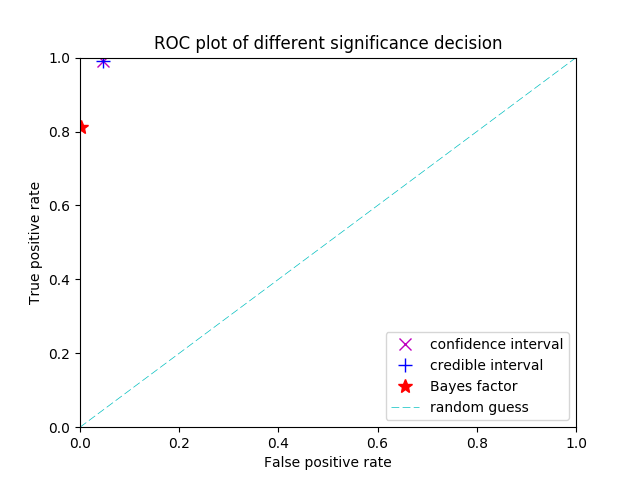
\includegraphics[scale=.6]{roc_sim_data.png}
\caption{ROC plot on simulation data}
\label{fig:roc_sim_data}
\end{figure}

Next, we show the results of \textbf{early stopping} algorithms in the following table . To make notations compact, we use FPR for false positive rate, RTR (all) for run time reduced (all), RTR (TP) for run time reduced (true positive) and CI for confidence interval. The definition of each metric is described previously in Section ~\ref{sec:esc}.

\begin{center}
  \begin{tabular}{ | r | r | c | c | c | c | c | }
    \hline
    \textbf{Significance} & \textbf{Early Stopping}  & \textbf{Paradigm} & \textbf{FPR} & \textbf{RTR(all)} & \textbf{RTR(TP)} & \textbf{Bias} \\ \hline\hline
    CI &  CI & frequentist & 3.3\% &  1.60\% & 16.74\% & 0.00 \\ \hline
    Credible Interval & Credible Interval & Bayesian & \textbf{22.6}\% & 17.56\% &  42.28\% & 0.00 \\ \hline
    Bayes factor & Bayes factor & Bayesian & 0.7\% & 0.57\% & 42.5\% & -0.02 \\ \hline
    Bayes factor & Bayes precision & Bayesian & 0.2\% & 78.02\% &  78.02\% &  0.00 \\ \hline
  \end{tabular}
\captionof{table}{Performance of early stopping in A/A test on simulation data}
\end{center}

\begin{center}
  \begin{tabular}{ | r | r | c | c | c | c | c | }
    \hline
    \textbf{Significance} & \textbf{Early Stopping}  & \textbf{Paradigm} & \textbf{FPR} & \textbf{RTR(all)} & \textbf{RTR(TP)} & \textbf{Bias} \\ \hline\hline
    CI &  CI & frequentist &1.7\% & 51.58\% & 51.74\% & -0.01 \\ \hline
    Credible Interval & Credible Interval & Bayesian & 0.7\% & 78.53\% & 78.78\% & 0.00 \\ \hline
    Bayes factor & Bayes factor & Bayesian & 7.8\% & 46.44\% & 52.96\% & 0.00 \\ \hline
    Bayes factor & Bayes precision & Bayesian & \textbf{67.8}\% & 77.95\% & 77.76\% & -0.02 \\ \hline
  \end{tabular}
\captionof{table}{Performance of early stopping on simulation data}
\end{center}

Note that false positive rate is the most critical metric when evaluating early stopping. This is because it makes no sense how much run time we have saved, if we stop the test with a wrong conclusion.

We observe that there is a large false positive rate by credible interval on A/A tests and also by Bayes precision on A/B tests. It would be dangerous to roll these two methods out in production without further study. In general, the confidence interval approach works best on simulation data.


\subsection{Real Data}
We first fetch raw data in BigQuery from previous A/B testings. After some cleanup and data processing, we got 10 datasets with nice properties for evaluating A/B testing. You can download processed datasets in my \href{https://github.com/shansfolder/ABTestingEarlyStoppingEvaluation/tree/master/data/real/processed}{\underline{GitHub repository}}. For a compact notation, we refer to each dataset using the following abbreviation.
\begin{itemize}[noitemsep]
\item DTP\_CH\_web (\textbf{DTP})
\item Editorial\_Assortment\_Entries\_treatment1 (\textbf{EAE1})
\item Editorial\_Assortment\_Entries\_treatment2 (\textbf{EAE2})
\item Editorial\_Catalog\_entries\_Msite (\textbf{ECEM})
\item lipstick\_catalog\_naviTracking\_bunchbox\_IT (\textbf{LCIT})
\item lipstick\_catalog\_naviTracking\_bunchbox\_NL (\textbf{LCNL})
\item segmented\_sorting\_fasion\_floor\_fashion (\textbf{FFF})
\item segmented\_sorting\_fasion\_floor\_modern (\textbf{FFM})
\item segmented\_sorting\_fasion\_floor\_no\_floor (\textbf{FFNF})
\item segmented\_sorting\_fasion\_floor\_trend (\textbf{FFT})
\end{itemize}

We test early stopping algorithms with the most frequently used primary KPI in the past, which is \textbf{conversion rate per session (CR)}.

A summary of dataset properties can be found below, where \textbf{traffic split} represents the percentage of samples in treatment group, and \textbf{NaN in CR} represents the percentage of missing values after computing conversion rate per session.

\begin{center}
  \begin{tabular}{ | l | c | r | r | r | c | c |}
    \hline
    \textbf{Dataset} & \textbf{\#Days}  & \textbf{\#Samples} & \textbf{\#Control} & \textbf{\#Treatment} &  \textbf{Traffic Split} & \textbf{NaN in CR} \\ \hline\hline
     DTP & 20 & 552995 & 284448 & 268547 & 48.56\% & 1.84\% \\ \hline
     EAE1 & 21 & 329960 & 164833 & 165127 & 50.04\% & 0.00\% \\ \hline
     EAE2 & 21 & 329910 & 164833 & 165077 & 50.04\% & 0.00\% \\ \hline
     ECEM & 35 & 250186 & 126106 & 124080 & 49.60\% & \textbf{7.83\%} \\ \hline
     LCIT & 14 & 970017 & 485157 & 484860 & 49.98\% & 0.00\% \\ \hline
     LCNL & 14 & \textbf{1027470} & 513266 & 514204 & 50.05\% & 0.00\% \\ \hline
     FFF & \textbf{56} & 135995 & 68855 & 67140 & 49.37\% & 0.00\% \\ \hline
     FFM & \textbf{56} & 68596 & 34778 & 33818 & 49.30\% & 0.00\% \\ \hline
     FFNF & \textbf{56} & 134800 & 67583 & 67217 & 49.86\% & 0.00\% \\ \hline
     FFT & \textbf{56} & 34265 & 16776 & 17489 & 51.04\% & 0.00\% \\ \hline
  \end{tabular}
\captionof{table}{Properties of selected real-world datasets for evaluation}
\end{center}

The \textbf{conversion rate per session} for visit $i$ is calculated as simple as $CR_i = \frac{O_i}{S_i}$, where $O_i$ is the sum of orders during visit $i$, and $S_i$ is the number of sessions during visit $i$.

Given $n$ samples of visits, it is worth noting that there are two ways to compute the overall conversion rate, we can calculate the average ratio per entity, i.e.
\begin{align} 
\begin{split}
CR^{(pe)} = \frac{1}{n} \sum_{i=1}^{n} CR_i = \frac{1}{n} \sum_{i=1}^{n} \frac{O_i}{S_i}
\end{split}					
\end{align}

This approach assumes equal weights on the contribution of each visit, which might lead to huge bias in practice. In fact, the product analysts in Zalando use the ratio of totals to reflect overall equal contributions to the conversion rate, which can be formulated as:
\begin{align} 
\begin{split}
CR^{(rt)} = \frac{\sum_{i=1}^{n}O_i}{\sum_{i=1}^{n}S_i} 
\end{split}					
\end{align}

Nevertheless, this will just be one value in the end. Our statistical hypothesis requires that we have a group of samples in both control and treatment group.
To be able to have samples of $CR^{(rt)}$ from $CR^{(pe)}$, we implemented a re-weighting trick (proof is trivial):
\begin{align} 
\begin{split}
CR^{(rt)} = \frac{1}{n} \sum_{i=1}^{n} \alpha_i \frac{O_i}{S_i}
\end{split}					
\end{align}
where
\begin{align} 
\begin{split}
\alpha_i  = n \frac{S_i}{\sum_{i=1}^{n} S_i}
\end{split}					
\end{align}

Now that we have seen all components to evaluate real-world usecases, we can show the result of performance on real data. It is illustrated in the table below.

\begin{center}
  \begin{tabular}{ | c | p{30mm} | p{30mm} | p{30mm} | p{30mm} |}
    \hline
     Dataset & Frequentist  & Credible Interval & Bayes Factor & Bayes Precision \\ \hline\hline
     DTP & Correctly stopped: saved 35\% time & Correctly stopped: saved 65\% time & Correctly stopped: saved 20\% time & \textbf{Wrongly} stopped \\ \hline
     EAE1 & No stop & \textbf{Wrongly} stopped & No stop & Correctly stopped: saved 95\% time \\ \hline
     EAE2 & No stop & Correctly stopped: saved 95\% time & No stop & Correctly stopped: saved 95\% \\ \hline
     ECEM & No stop & No stop & No stop & Correctly stopped: saved 94\% time \\ \hline
     LCIT & No stop & & & \\ \hline
     LCNL & No stop & & & \\ \hline
     FFF & Correctly stopped: saved 1\% time & Correctly stopped: saved 79\% time & No stop & Correctly stopped: saved 91\% time \\ \hline
     FFM & No stop & No stop & No stop & Correctly stopped: saved 84\% time \\ \hline
     FFNF & No stop & \textbf{Wrongly} stopped & No stop & Correctly stopped: saved 91\% time\\ \hline
     FFT & No stop & No stop & No stop & Correctly stopped: saved 70\% time \\ \hline
  \end{tabular}
\captionof{table}{Performance of early stopping on real data}
\end{center}


\section{Conclusion}
Given bad performance of Bayes precision and credible interval on both simulation data and real data, we will need to investigate further on the theory and implementation of these two methods.

Bayes factors and the frequentist approach both perform good. However, we need to change the whole concept of our A/B testing to roll out the Bayesian approach in live system. Therefore, we suggest the frequentist approach --- i.e., use group sequential method for early stopping and confidence interval for significance decision.

%----------------------------------------------------------------------------------------

\end{document}